\chapter{Creare una animazione}
{ }\hfill\textbf{Livello:} Medio\\
Questo capitolo presenta due differenti temi con l'obiettivo di creare animazioni in \xlogo.


\section{Le cifre della calcolatrice}
\begin{center}
	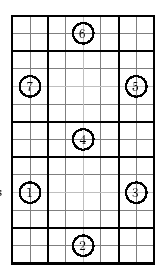
\includegraphics{pics/animation-chiffre.png}
\end{center}

Questo tema è basato sul fatto che tutte le cifre delle calcolatrici potrebbero essere disegnate secondo lo schema qui sopra. Per esempio per disegnare la cifra 4 illuminiamo i rettangoli 3,4,5,7. Per disegnare la cifra 8, illuminiamo tutti i rettangoli. Per disegnare la cifra 3 illuminiamo i rettangoli 2,3,4,5,6.

\subsection{Riempire un rettangolo}
\begin{center}
	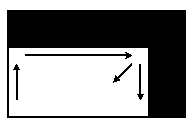
\includegraphics{pics/animation-rectangle.png}
\end{center}
Se vogliamo disegnare un rettangolo colorato di dimensioni 100 per 200 una prima possibilità potrebbe essere di disegnare un rettangolo vuoto di 100x200, quindi un altro rettangolo di 99x199 e così via\textellipsis fino a che il rettangolo sarà completamente pieno.\\
Cominciamo definendo un rettangolo con due variabili corrispondenti alla base ed alla altezza.
\begin{lstlisting}[caption="Un semplice rettangolo dati i due lati"]
Per rec :h :w
	Ripeti 2[Av :h DX 90 Av :w DX 90]
Fine
\end{lstlisting}

Per riempire un rettangolo dobbiamo scrivere:\\
\texttt{rec 100 200 rec 99 199 rec 98 198  ..... rec 1 101}\\ \\
Definiamo quindi una procedura per questo rettangolo riempito.
\begin{lstlisting}[caption="Un rettangolo colorato"]
Per rettangolo :h :w
	rec :h :w
	rettangolo :h-1 :w-1
Fine
\end{lstlisting}

Verifichiamo con \texttt{rettangolo 100 200} e capiamo che c'è un problema. La procedura non si ferma dopo aver riempito tutto il rettangolo. Dobbiamo inserire un comando di uscita che capisca quando la base o l'altezza diventano 0. Quando si realizza questa condizione il programma si deve fermare con la primitiva \texttt{Ferma}.
\begin{lstlisting}[caption="Una migliore implementazione del rettangolo colorato"]
Per rettangolo :h :w
	Se o :h=0 :w=0 [Ferma]
	rec :h :w
	rettangolo :h-1 :w-1
Fine
\end{lstlisting}

Invece di usare la primitiva \texttt{o} è possibile usare il simbolo ``|'', la riga 2 diventa: \lstinline!Se :h=0 | :w=0 [Ferma]!.


\subsection{Il programma}
Dobbiamo riutilizzare il precedente rettangolo riempito. Supponiamo che la tartaruga comincia dall'angolo in basso a sinistra. Definiamo una procedura chiamata \texttt{numero} che accetta 7 argomenti: \texttt{:a}, \texttt{:b}, \texttt{:c}, \texttt{:d}, \texttt{:e}, \texttt{:f}, \texttt{:g}. Quando \texttt{:a} è uguale a 1 disegniamo il rettangolo 1. Se \texttt{:a} è uguale a 0 non disegniamo alcun rettangolo. Questa è la idea principale.\\
\textbf{Il programma}:
\begin{lstlisting}[caption="Disegnare un numero fatto di rettangoli"]
Per numero :a :b :c :d :e :f :g
# disegniamo il rettangolo 1
Se :a=1 [rettangolo 160 40]
# disegniamo il rettangolo 2
Se :b=1 [rettangolo 40 160]
PennaSu DX 90 Avanti 120 SX 90 PennaGiu
# disegniamo il rettangolo 3
Se :c=1 [rettangolo 160 40]
PennaSu Avanti 120 PennaGiu
# disegniamo il rettangolo 5
Se :e=1 [rettangolo 160 40]
# disegniamo il rettangolo 4
SX 90 PennaSu Indietro 40 PennaGiu
Se :d=1 [rettangolo 160 40]
# disegniamo il rettangolo 6
DX 90 PennaSu Avanti 120 SX 90 PennaGiu
Se :f=1 [rettangolo 160 40]
# disegniamo il rettangolo 7
PennaSu Avanti 120 SX 90 Indietro 40 PennaGiu 
Se :g=1 [rettangolo 160 40]
end
\end{lstlisting}


\subsection{Creare l'animazione}
In questa parte definiamo il conteggio a rovescio da 9 a 0.

\begin{lstlisting}[caption="Conteggio a rovescio da 9 a 0"]
Per countd
	PulisciSchermo NascondiTartaruga numero 0 1 1 1 1 1 1 Aspetta 60
	PulisciSchermo NascondiTartaruga numero 1 1 1 1 1 1 1 Aspetta 60
	PulisciSchermo NascondiTartaruga numero 0 0 1 0 1 1 0 Aspetta 60
	PulisciSchermo NascondiTartaruga numero 1 1 1 1 0 1 1 Aspetta 60
	PulisciSchermo NascondiTartaruga numero 0 1 1 1 0 1 1 Aspetta 60
	PulisciSchermo NascondiTartaruga numero 0 0 1 1 1 0 1 Aspetta 60
	PulisciSchermo NascondiTartaruga numero 0 1 1 1 1 1 0 Aspetta 60
	PulisciSchermo NascondiTartaruga numero 1 1 0 1 1 1 0 Aspetta 60
	PulisciSchermo NascondiTartaruga numero 0 0 1 0 1 0 0 Aspetta 60
	PulisciSchermo NascondiTartaruga numero 1 1 1 0 1 1 1 Aspetta 60
Fine
\end{lstlisting}

C'è un piccolo problema, un effetto di sfarfallamento durante il disegno di ciascuna cifra. Per rendere l'animazione più fluida useremo la modalità di animazione mediante tre primitive:
\begin{itemize}
	\item \texttt{Animazione} permette di entrare nella modalità animazione. La tartaruga smette di disegnare sull'area di disegno ma si ricorda di tutti i cambiamenti. Per visualizzare l'immagine è necessario usare la primitiva \texttt{Ridisegna}.
	\item  \texttt{FermaAnimazione} restituisce la modalità classica.
\end{itemize}

Modifichiamo il programma in questo modo:
\begin{lstlisting}[caption="Animazione del conteggio a rovescio da 9 a 0"]
Per countd
	Animazione
	PulisciSchermo NascondiTartaruga numero 0 1 1 1 1 1 1 Ridisegna Aspetta 60
	PulisciSchermo NascondiTartaruga numero 1 1 1 1 1 1 1 Ridisegna Aspetta 60
	PulisciSchermo NascondiTartaruga numero 0 0 1 0 1 1 0 Ridisegna Aspetta 60
	PulisciSchermo NascondiTartaruga numero 1 1 1 1 0 1 1 Ridisegna Aspetta 60
	PulisciSchermo NascondiTartaruga numero 0 1 1 1 0 1 1 Ridisegna Aspetta 60
	PulisciSchermo NascondiTartaruga numero 0 0 1 1 1 0 1 Ridisegna Aspetta 60
	PulisciSchermo NascondiTartaruga numero 0 1 1 1 1 1 0 Ridisegna Aspetta 60
	PulisciSchermo NascondiTartaruga numero 1 1 0 1 1 1 0 Ridisegna Aspetta 60
	PulisciSchermo NascondiTartaruga numero 0 0 1 0 1 0 0 Ridisegna Aspetta 60
	PulisciSchermo NascondiTartaruga numero 1 1 1 0 1 1 1 Ridisegna Aspetta 60
	FermaAnimazione
Fine
\end{lstlisting}



\section{L'uomo che cresce}
\begin{center}
	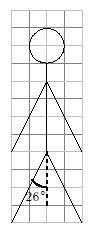
\includegraphics{pics/animation-bonhomme.png}
\end{center}
Come prima cosa definiamo una procedura \texttt{uomo} che disegna lo schema qui sopra. Usiamo una variabile per riprodurlo a scale diverse.
\begin{lstlisting}[caption="Disegno di un uomo stilizzato"]
Per uomo :c
	SX 154 Avanti 44*:c Indietro 44*:c 
	SX 52 Avanti 44*:c Indietro 44*:c 
	SX 154 Avanti 40*:c
	SX 154 Avanti 44*:c Indietro :c*44 
	SX 52 Avanti 44*:c Indietro :c*44 
	SX 154 Avanti 10*:c
	SX 90 Ripeti 180[Avanti :c/2 DX 2] DX 90
Fine
\end{lstlisting}


Adesso creiamo una animazione che farà crescere l'uomo. Per realizzare ciò disegniamo \texttt{uomo 0.1}, quindi \texttt{uomo 0.2}, \texttt{uomo 0.3}\textellipsis fino a \texttt{uomo 5}. Fra ciascun uomo cancelliamo l'area di disegno. Otteniamo due diverse procedure:
\begin{lstlisting}[caption="Disegno di un uomo che cresce"]
Per uomo :c
	SX 154 Avanti 44*:c Indietro 44*:c 
	SX 52 Avanti 44*:c Indietro 44*:c 
	SX 154 Avanti 40*:c
	SX 154 Avanti 44*:c Indietro :c*44 
	SX 52 Avanti 44*:c Indietro :c*44 
	SX 154 Avanti 10*:c
	SX 90 Ripeti 180[Avanti :c/2 DX 2] DX 90
	Se :c=5[Ferma]
	PulisciSchermo NascondiTartaruga uomo :c+0.1
Fine

Per via
	PulisciSchermo NascondiTartaruga
	uomo 0
Fine
\end{lstlisting}

Alla fine per rendere l'animazione fluida useremo la modalità animazione e la primitiva \texttt{Ridisegna}.
\begin{lstlisting}[caption="Animazione di un uomo che cresce"]
Per uomo :c
	SX 154 Avanti 44*:c Indietro 44*:c 
	SX 52 Avanti 44*:c Indietro 44*:c 
	SX 154 Avanti 40*:c
	SX 154 Avanti 44*:c Indietro :c*44 
	SX 52 Avanti 44*:c Indietro :c*44 
	SX 154 Avanti 10*:c
	SX 90 Ripeti 180[Avanti :c/2 DX 2] DX 90
	Ridisegna
	Se :c=5[Ferma]
	PulisciSchermo NascondiTartaruga uomo :c+0.1
Fine

Per via
	PulisciSchermo NascondiTartaruga Animazione
	uomo 0
	FermaAnimazione
Fine
\end{lstlisting}

\textbf{Nota}: qui la procedura \texttt{uomo} è ricorsiva. Avremmo anche potuto usare la  primitiva \texttt{RipetiPer} per assegnare alla variabile :c i valori da 0.1 a 5, in questo modo:
\begin{lstlisting}[caption="Animazione non ricorsiva di un uomo che cresce"]
Per uomo :c
	PulisciSchermo SX 154 Avanti 44*:c Indietro 44*:c 
	SX 52 Avanti 44*:c Indietro 44*:c 
	SX 154 Avanti 40*:c
	SX 154 Avanti 44*:c Indietro :c*44 
	SX 52 Avanti 44*:c Indietro :c*44 
	SX 154 Avanti 10*:c
	SX 90 Ripeti 180[Avanti :c/2 DX 2] DX 90
	Ridisegna
Fine

Per go
	NascondiTartaruga Animazione
	RipetiPer [c 0 5 0.1][uomo :c]
	FermaAnimazione
Fine
\end{lstlisting}